\documentclass{aastex61}


%% arguement options are:
%%
%%  twocolumn   : two text columns, 10 point font, single spaced article.
%%                This is the most compact and represent the final published
%%                derived PDF copy of the accepted manuscript from the publisher
%%  manuscript  : one text column, 12 point font, double spaced article.
%%  preprint    : one text column, 12 point font, single spaced article.  
%%  preprint2   : two text columns, 12 point font, single spaced article.
%%  modern      : a stylish, single text column, 12 point font, article with
%% 		  wider left and right margins. This uses the Daniel
%% 		  Foreman-Mackey and David Hogg design.
%%
%% Note that you can submit to the AAS Journals in any of these 6 styles.
%%
%% There are other optional arguments one can envoke to allow other stylistic
%% actions. The available options are:
%%
%%  astrosymb    : Loads Astrosymb font and define \astrocommands. 
%%  tighten      : Makes baselineskip slightly smaller, only works with 
%%                 the twocolumn substyle.
%%  times        : uses times font instead of the default
%%  linenumbers  : turn on lineno package.
%%  trackchanges : required to see the revision mark up and print its output
%%  longauthor   : Do not use the more compressed footnote style (default) for 
%%                 the author/collaboration/affiliations. Instead print all
%%                 affiliation information after each name. Creates a much
%%                 long author list but may be desirable for short author papers
%%
%% these can be used in any combination, e.g.
%%
%% \documentclass[twocolumn,linenumbers,trackchanges]{aastex61}

\usepackage{graphicx}
\usepackage{amssymb}
\usepackage{color}
\usepackage{breakurl}

\usepackage{amsthm, amsmath}
\def\UrlFont{\sf}
\let\captionbox\relax
\usepackage[caption=false]{subfig}

\usepackage{tikz}
\usetikzlibrary{decorations.markings}


%% Definitions for the journal names
%\newcommand{\adv}{    {\it Adv. Space Res.}} 
%\newcommand{\annG}{   {\it Ann. Geophys.}} 
%\newcommand{\aap}{    {\it Astron. Astrophys.}}
%\newcommand{\aaps}{   {\it Astron. Astrophys. Suppl.}}
%\newcommand{\aapr}{   {\it Astron. Astrophys. Rev.}}
%\newcommand{\ag}{     {\it Ann. Geophys.}}
%\newcommand{\aj}{     {\it Astron. J.}} 
%\newcommand{\apj}{    {\it Astrophys. J.}}
%\newcommand{\apjl}{   {\it Astrophys. J. Lett.}}
%\newcommand{\apss}{   {\it Astrophys. Space Sci.}} 
%\newcommand{\cjaa}{   {\it Chin. J. Astron. Astrophys.}} 
%\newcommand{\gafd}{   {\it Geophys. Astrophys. Fluid Dyn.}}
%\newcommand{\grl}{    {\it Geophys. Res. Lett.}}
%\newcommand{\ijga}{   {\it Int. J. Geomagn. Aeron.}}
%\newcommand{\jastp}{  {\it J. Atmos. Solar-Terr. Phys.}} 
%\newcommand{\jgr}{    {\it J. Geophys. Res.}}
%\newcommand{\lrsp}{Living Rev. Solar Phys.}
%\newcommand{\mnras}{  {\it Mon. Not. Roy. Astron. Soc.}}
%\newcommand{\nat}{    {\it Nature}}
%\newcommand{\pasp}{   {\it Pub. Astron. Soc. Pac.}}
%\newcommand{\pasj}{   {\it Pub. Astron. Soc. Japan}}
%\newcommand{\pre}{    {\it Phys. Rev. E}}
%\newcommand{\solphys}{{\it Solar Phys.}}
%\newcommand{\sovast}{ {\it Soviet  Astron.}} 
%\newcommand{\ssr}{    {\it Space Sci. Rev.}}


%\received{July 1, 2016}
%\revised{September 27, 2016}
%\accepted{\today}
%\submitjournal{ApJ}


%%%%%%%%%%%%%%%%%%%%%%%%%%%%%%%%%%%%%%%%%%%%%%%%%%%%%%%%%%%%%%%%%%%%%%%%%%%%%%%%
%%
\shorttitle{Evolution of Asymmetric MHD Waves}
\shortauthors{Allcock and Erd\'{e}lyi}
\watermark{DRAFT}
%%
%%%%%%%%%%%%%%%%%%%%%%%%%%%%%%%%%%%%%%%%%%%%%%%%%%%%%%%%%%%%%%%%%%%%%%%%%%%%%%%%

\begin{document}
\title{Evolution of Asymmetric Slab Magnetohydrodynamic Waves}

%% LaTeX will automatically break titles if they run longer than
%% one line. However, you may use \\ to force a line break if
%% you desire. In v6.1 you can include a footnote in the title.

%% A significant change from earlier AASTEX versions is in the structure for 
%% calling author and affilations. The change was necessary to implement 
%% autoindexing of affilations which prior was a manual process that could 
%% easily be tedious in large author manuscripts.
%%
%% The \author command is the same as before except it now takes an optional
%% arguement which is the 16 digit ORCID. The syntax is:
%% \author[xxxx-xxxx-xxxx-xxxx]{Author Name}
%%
%% This will hyperlink the author name to the author's ORCID page. Note that
%% during compilation, LaTeX will do some limited checking of the format of
%% the ID to make sure it is valid.
%%
%% Use \affiliation for affiliation information. The old \affil is now aliased
%% to \affiliation. AASTeX v6.1 will automatically index these in the header.
%% When a duplicate is found its index will be the same as its previous entry.
%%
%% Note that \altaffilmark and \altaffiltext have been removed and thus 
%% can not be used to document secondary affiliations. If they are used latex
%% will issue a specific error message and quit. Please use multiple 
%% \affiliation calls for to document more than one affiliation.
%%
%% The new \altaffiliation can be used to indicate some secondary information
%% such as fellowships. This command produces a non-numeric footnote that is
%% set away from the numeric \affiliation footnotes.  NOTE that if an
%% \altaffiliation command is used it must come BEFORE the \affiliation call,
%% right after the \author command, in order to place the footnotes in
%% the proper location.
%%
%% Use \email to set provide email addresses. Each \email will appear on its
%% own line so you can put multiple email address in one \email call. A new
%% \correspondingauthor command is available in V6.1 to identify the
%% corresponding author of the manuscript. It is the author's responsibility
%% to make sure this name is also in the author list.
%%
%% While authors can be grouped inside the same \author and \affiliation
%% commands it is better to have a single author for each. This allows for
%% one to exploit all the new benefits and should make book-keeping easier.
%%
%% If done correctly the peer review system will be able to
%% automatically put the author and affiliation information from the manuscript
%% and save the corresponding author the trouble of entering it by hand.

\correspondingauthor{Robert Erd\'{e}lyi}
\email{robertus@sheffield.ac.uk}

\author[0000-0002-0771-743X]{Matthew Allcock}
\affil{Solar Physics and Space Plasma Research Centre, School of Mathematics and Statistics, University of Sheffield, Hicks Building, Hounsfield Road, Sheffield, S3 7RH, UK}

\author[0000-0003-3439-4127]{Robert Erd\'{e}lyi}
\affiliation{Solar Physics and Space Plasma Research Centre, School of Mathematics and Statistics, University of Sheffield, Hicks Building, Hounsfield Road, Sheffield, S3 7RH, UK}


\begin{abstract}

Abstract (250 word limit for ApJ)

\end{abstract}

\keywords{magnetohydrodynamics --- plasmas --- Sun: atmosphere --- Sun: oscillations --- waves}

\section{Introduction} \label{sec:intro}
Numerical results: \cite{ter_etal06}

Physicality of the principle leaky kink mode: \cite{cal03} solved the initial value problem of transverse waves in a cold magnetic flux tube. \cite{rud_etal06} repeated it showing PLK modes are on an unphysical banch of the complex plane (?). Commented on by \cite{cal06} and in return by \cite{rud_etal06b}. Settled (?) by considering numerical solution by \cite{ter_etal07} and analytically by \cite{and_etal07}. So PLK modes are not physical.

\section{Initial value problem - incompressible magnetic slab}

Consider an equilibrium plasma with magnetic field $B_0(x)\mathbf{\hat{z}}$, density $\rho_0(x)$, and pressure $p_0(x)$, without gravity. In the absence of structuring in the $z$-direction and considering perturbations in the $(x,z)$-plane only, we can take Fourier components for velocity and other parameters like $\mathbf{v}(\mathbf{x},t) = \mathbf{\hat{v}}(x)e^{i(kz + ly - \omega t)}$. The velocity perturbation amplitude in the inhomogeneous direction of an ideal plasma is given by
\begin{equation}
\frac{d}{dx}\left(\frac{\epsilon(x)}{l^2 + m_0^2(x)} \frac{d\hat{v}_x}{dx}\right) - \epsilon(x)\hat{v}_x = 0,
\label{gov gen}
\end{equation}
where
\begin{equation}
\epsilon(x) = \rho_0(x)[k^2v_A^2(x)-\omega^2], \quad
m_0^2(x) = \frac{(k^2c_0^2(x) - \omega^2)(k^2v_A^2(x) - \omega^2)}{(c_0^2(x) + v_A^2(x))(k^2c_T^2(x) - \omega^2)},
\end{equation}
and
\begin{equation}
c_0(x) = \sqrt{\frac{\gamma p_0(x)}{\rho_0(x)}}, \quad
v_A(x) = \frac{B_0(x)}{\sqrt{\mu \rho_0(x)}}, \quad
c_T(x) = \frac{c_0(x)v_A(x)}{\sqrt{c_0^2(x) + v_A^2(x)}}
\end{equation} are the sound, Alfv\'{e}n, and tube speeds, respectively.

When the plasma is incompressible, so that $c_0 \to \infty$, we have $c_T^2 \to v_A^2$ and $m_0^2 \to k^2$. After restricting the analysis to propagation only parallel to the magnetic field ($l = 0$), Equation~\eqref{gov gen} reduces to
\begin{equation}
\frac{d}{dx}\left(\epsilon(x) \frac{d\hat{v}_x}{dx}\right) - k^2\epsilon(x)\hat{v}_x = 0,
\label{gov}
\end{equation}
which is commonly used for solving eigenmode problems in MHD wave physics. In the present work, the temporal evolution of linear asymmetric MHD waves is considered so we must dial back our assumptions about how the wave behaviour changes through time.

Above we have used a Fourier decomposition in both space and time. To investigate the temporal evolution of solutions, we take only Fourier components in the $z$-direction, that is $\mathbf{v}(\mathbf{x},t) = \mathbf{\hat{v}}(x,t)e^{ikz}$, and we take the Laplace transform with respect to time, such that
\begin{equation}
\mathbf{\tilde{v}}(x) = \mathcal{L}\{\mathbf{\hat{v}}(x, t)\} = \int_0^\infty \mathbf{\widehat{v}}(x,t)e^{i\omega t} dt.
\end{equation}
This gives us the initial-value form of Equation~\eqref{gov} to be
\begin{equation}
\frac{d}{dx}\left(\epsilon(x) \frac{d\tilde{v}_x}{dx}\right) - k^2\epsilon(x)\tilde{v}_x = f(x, \omega),
\label{ivp gov}
\end{equation}
where
\begin{equation}
f(x, \omega) = ik\left\{\rho_0\left[\frac{\partial\hat{\Omega}}{\partial t}(x,0) - i\omega\hat{\Omega}(x,0)\right] - \left[\frac{\partial\hat{v}_z}{\partial t}(x,0) - i\omega \hat{v}_z(x,0)\right]\frac{d\rho_0}{dx}\right\},
\label{f}
\end{equation}
where the vorticity, $\Omega(x,t)\mathbf{\hat{y}} = \hat{\Omega}(x,t)e^{ikz}\mathbf{\hat{y}} = \nabla \times \mathbf{v}(\mathbf{x},t)$, is given by
\begin{equation}
\hat{\Omega}(\mathbf{x},t) = -\frac{i}{k}\left(\frac{\partial^2\hat{v}_x}{\partial x^2} - k^2 \hat{v}_x\right).
\end{equation}
(this differs from \cite{rae_etal81} by a factor of $-1$ due to taking Fourier forms like $e^{ikz}$ rather than $e^{-ikz}$). For utility later on, we define $\Psi_0 = \Psi(x, 0)$ by function $\Psi(x, t) = k(\rho_0\hat{\Omega}(x, t) - \rho_0'\hat{v}_z(x, t))$ so that $f(x, \omega) = \omega \Psi_0 + i\frac{\partial \Psi_0}{\partial t}$.

Consider equilibrium magnetic field and density profiles given by
\begin{equation}
B(x)=
\begin{cases}
B_1, & \text{if  }x<-x_0, \\
B_0, & \text{if }|x|\leq{x_0}, \\
B_2, & \text{if  }x>x_0,
\end{cases}
\quad \text{and} \quad
\rho(x)=
\begin{cases}
\rho_1, & \text{if  }x<-x_0, \\
\rho_0, & \text{if }|x|\leq{x_0}, \\
\rho_2, & \text{if  }x>x_0,
\end{cases}
\end{equation}
where $B_i$ and $\rho_i$ are uniform for $i = 0,1,2$. This establishes the plasma as magnetic slab embedded in an asymmetric magnetic background. So that the structure is in equilibrium, we require that the total pressure in each of the three regions be equal, that is
\begin{align}
p_1 + \frac{B_1^2}{2\mu} &= p_0  + \frac{B_0^2 }{2\mu} = p_2 + \frac{B_2^2 }{2\mu}, \label{eq:pressure}
\end{align}
where $p_i$ is the gas pressure in region $i$ and $\mu$ is the permeability of free space. The sound speed in each region is $c_i = \sqrt{\gamma p_i / \rho_i}$, for $i = 0, 1, 2$, where $\gamma$ is the adiabatic index. The Alfvén speed is denoted by $v_{Ai}= B_i/\sqrt{\rho_i \mu}$, for $i=0,1,2$. Equation~\ref{eq:pressure} describing equilibrium pressure balance yields the following relationship between the density ratios and characteristic speeds for any two regions,
\begin{align}
\frac{\rho_i}{\rho_j}= \frac{c_j^2 + \frac{1}{2} \gamma v_{Aj}^2}{c_i^2 + \frac{1}{2} \gamma v_{Ai}^2}, \quad \text{where} \quad i=0,1,2; \quad j=0,1,2; \quad i \neq j. \label{eq:ratio}
\end{align}

In this equilibrium, transverse velocity perturbations are related to initial perturbations in the following way:
\begin{equation}
\frac{d^2\tilde{v}_x}{dx^2} - k^2\tilde{v}_x = 
\begin{cases}
f(x, \omega)/\epsilon_1, & \text{if  } x<-x_0,\\
f(x, \omega)/\epsilon_0, & \text{if  } |x|<x_0,\\
f(x, \omega)/\epsilon_2, & \text{if  } x>x_0,
\end{cases}
\label{ivp gov slab 2}
\end{equation}
under the boundary conditions $\tilde{v}_x(-x_0) = \tilde{A}_1$ and $\tilde{v}_x(x_0) = \tilde{A}_2$.

Sturm-Liouville Theory tells us that the Green's function, $G(x;s)$, corresponding to Equation~\eqref{ivp gov slab 2} must satisfy 
\begin{equation}
\frac{\partial^2G}{\partial x^2} - k^2 G = \delta(x-s), \quad G(-x_0;s) = G(x_0;s) = 0,
\end{equation}
where $\delta$ denotes the Dirac Delta function. It is instructive to piecewise define the Green's function as
\begin{equation}
G(x;s) = 
\begin{cases}
G_1(x;s), & \text{if } x < -x_0, \\
G_0(x;s), & \text{if } |x| < x_0, \\
G_2(x;s), & \text{if } x_0 < x.
\end{cases}
\end{equation}
The general solution, for $|x| < x_0$, of the equation for $G_0$ is
\begin{equation}
G_0(x;s) = c_1\sinh(k(x - x_0)) + c_2\sinh(k(x + x_0)),
\end{equation}
where $c_1 = 0$ for $x < s$ and $c_2 = 0$ for $x > s$. In accordance with standard Green's Functions procedure \citep{boy_etal12}, ensuring $G_0$ and $\partial G_0 / \partial x$ have jumps of 0 and 1 at $x = s$, respectively,  determines $c_1$ and $c_2$, so that $G_0(x;s)$ is
\begin{equation}
G_0(x;s) = \frac{1}{k\sinh(2k x_0)}
\begin{cases}
\sinh(k(s - x_0))\sinh(k(x + x_0)), & \text{if } -x_0<x<s, \\
\sinh(k(x - x_0))\sinh(k(s + x_0)), & \text{if } s<x<x_0.
\end{cases}
\end{equation}

Because the boundary conditions are inhomogeneous, we must add to the standard Green's function solution a term that is a solution to the homogeneous equation and the inhomogeneous boundary conditions. In this manner, we find that the solution within the slab is
\begin{equation}
\tilde{v}_x(x) = \frac{1}{\sinh{2kx_0}} \left[ \tilde{A}_1\sinh(k(x_0 - x)) + \tilde{A}_2\sinh(k(x_0 + x)) \right] + \frac{1}{\epsilon_0}\int_{-x_0}^{x_0} G_0(x;s) f(s, \omega) ds.
\end{equation}

Similarly, we find that the Green's function for the plasma outside the slab is 
\begin{equation}
G_1(x;s) = \frac{1}{k}
\begin{cases}
e^{k(x + x_0)}\sinh(k(s + x_0)), & \text{if } x < s, \\
e^{k(s + x_0)}\sinh(k(x + x_0)), & \text{if } s < x < -x_0,
\end{cases}
\end{equation}
for $x < -x_0$, and
\begin{equation}
G_2(x;s) = -\frac{1}{k}
\begin{cases}
e^{-k(s - x_0)}\sinh(k(x - x_0)), & \text{if } x_0 < x < s, \\
e^{-k(x - x_0)}\sinh(k(s - x_0)), & \text{if } s < x,
\end{cases}
\end{equation}
for $x > x_0$. Therefore the solution is
\begin{equation}
\tilde{v}_x(x) = \tilde{A}_1e^{k(x_0 + x)} + \frac{1}{\epsilon_1}\int_{-\infty}^{-x_0} G_1(x;s) f(s, \omega) ds,
\end{equation}
for $x < -x_0$, and
\begin{equation}
\tilde{v}_x(x) = \tilde{A}_2e^{k(x_0 - x)} + \frac{1}{\epsilon_2}\int_{x_0}^{\infty} G_2(x;s) f(s, \omega) ds,
\end{equation}
for $x > x_0$.


\subsection{Matching solutions}
To establish physically relevant solutions, we require that the transverse velocity and the total pressure are continuous over each interface. Given the above solutions, the transverse velocity is automatically continuous over the boundaries. The perturbation in the total pressure, $P_T$, for a compressible plasma is given (for example, in \cite{all_etal17}) by
\begin{equation}
\tilde{P}_T(x) = \frac{\Lambda}{m}\frac{d\tilde{v}_x}{d x},
\end{equation}
where
\begin{equation}
\Lambda = \frac{i\rho(\omega^2 - k^2v_A^2)}{m\omega},
\quad
m^2 = \frac{(k^2v_A^2 - \omega^2)(k^2c_0^2 - \omega^2)}{(c_0^2 + v_A^2)(k^2c_T^2 - \omega^2)},
\quad \text{and} \quad
c_T^2 = \frac{c_0^2 v_A^2}{c_0^2 + v_A^2}.
\end{equation}
When the plasma is incompressible, $m^2 \to k^2$, therefore continuity in total pressure is equivalent to continuity in $\epsilon(x)\tilde{v}_x'(x)$ for an incompressible plasma.

Applying this boundary condition gives
\begin{equation}
\tilde{A}_1(\omega) = \frac{T_1(\omega)}{k D(\omega)}, \quad \tilde{A}_2(\omega) = \frac{T_2(\omega)}{k D(\omega)},
\end{equation}
where
\begin{equation}
D(\omega) = \epsilon_0(\epsilon_1 + \epsilon_2)\cosh(2kx_0) + (\epsilon_0^2 + \epsilon_1\epsilon_2)\sinh(2kx_0)
\label{D incomp}
\end{equation}
is called the \textit{dispersion function} and $T_{1,2}$ are functionals given by
\begin{align}
T_1(\omega) &= T_1[f](\omega) = (I_0^- - I_1)[\epsilon_0\cosh(2kx_0) + \epsilon_2\sinh(2kx_0)] - \epsilon_0(I_0^+ + I_2), \\
T_2(\omega) &= T_2[f](\omega) = \epsilon_0(I_0^- - I_1) - (I_0^+ + I_2)[\epsilon_0\cosh(2kx_0) + \epsilon_1\sinh(2kx_0)],
\end{align}
where
\begin{align}
I_0^\pm &= I_0^\pm[f] = \int_{-x_0}^{x_0} \frac{\sinh(k(s \pm x_0))}{\sinh(2kx_0)} f(s, \omega) ds, \\
I_1 &= I_1[f] = \int_{-\infty}^{-x_0} e^{k(s + x_0)} f(s, \omega) ds,
\quad
I_2 = I_2[f] = \int_{x_0}^\infty e^{k(x_0 - s)} f(s, \omega) ds.
\end{align}


\subsection{Solution in time}

To recover the transverse velocity, $v_x(x, t)$, we employ the inverse Laplace transform (non-standard, discussed in Appendix~\ref{app: laplace trans}), such that
\begin{equation}
v_x(x,t) = \mathcal{L}^{-1}\{\tilde{v}_x(x, \omega)\} = \frac{1}{2\pi} \lim_{L \to \infty} \int_{i\gamma - L}^{i\gamma + L} \tilde{v}_x(x,\omega) e^{-i\omega t} d\omega,
\label{laplace transform}
\end{equation}
where $\gamma$ is a real number such that all the singularities of the integrand are below the contour of integration to ensure that all singularities contribute to the integral. The integral is evaluated along an infinite horizontal line in the upper half of the complex plane and is dependent on the singularities (with respect to $\omega$) of $\tilde{v}_x$, whose residues determine the value of the contour integral.

Focusing firstly on the region $x<-x_0$, the solution is
\newcommand{\e}{\epsilon}
\begin{align}
v_x &= \mathcal{L}^{-1} \left\{ \tilde{A}_1 e^{k(x+x_0)} + \frac{1}{\e_1} \int_{-\infty}^{-x_0} G_1(x;s)f(s, \omega)ds \right\}, \\
&= e^{k(x+x_0)} \mathcal{L}^{-1}\left\{ \tilde{A}_1 \right\} + \int_{-\infty}^{-x_0} G_1(x;s) \mathcal{L}^{-1}\left\{ \frac{f(s, \omega)}{\e_1} \right\} ds, \\
&= e^{k(x+x_0)} \mathcal{L}^{-1}\left\{ \tilde{A}_1 \right\} + \int_{-\infty}^{-x_0} G_1(x;s) \left[ \Psi (s, 0) \mathcal{L}^{-1}\left\{ \frac{\omega}{\e_1} \right\} + i \frac{\partial \Psi}{\partial t}(s, 0) \mathcal{L}^{-1}\left\{ \frac{1}{\e_1} \right\}\right] ds,
\label{sol incomp}
\end{align}

\textcolor{red}{CONSIDER ADDING AN OVERVIEW OF THE FOLLOWING METHOD TO EVALUATE THE INTEGRALS IN THE ABOVE.}

The first inverse Laplace transform (ILT), $\mathcal{L}^{-1}\left\{ \tilde{A}_1 \right\}$, in the above solution is calculated as follows. The functions $\epsilon_{0,1,2}$ are polynomial in $\omega$, and are therefore entire. The integrals $I_{1,2}$ and $I_0^\pm$ are not functions of $\omega$ so also contribute no singularities in $\omega$. Therefore, $T_1$ and $T_2$ are entire functions. Hence, 

The zeros of $D(\omega)$ are determined by firstly noting that $D=0$ is the dispersion relation of the corresponding eigenvalue problem solved by \cite{zsa_etal18}. They show that the dispersion relation governing transverse wave propagation parallel to the magnetic field in an asymmetric slab of compressible plasma is given by
\begin{equation}
2(\Lambda_0^2 + \Lambda_1 \Lambda_2) + \Lambda_0(\Lambda_1 + \Lambda_2)[\tanh(m_0x_0) + \coth(m_0x_0)] = 0,
\label{DR}
\end{equation}
where
\begin{equation}
\Lambda_j = -\frac{i\rho_j(k^2v_{Aj}^2 - \omega^2)}{\omega m_j},
\quad
m_j^2 = \frac{(k^2c_j^2 - \omega^2)(k^2v_{Aj}^2 - \omega^2)}{(c_j^2 + v_{Aj}^2)(k^2c_{Tj}^2 - \omega^2)},
\quad
\text{and}
\quad
c_{Tj}^2 = \frac{c_j^2v_{Aj}^2}{c_j^2 + v_{Aj}^2},
\end{equation}
for $j = 0, 1, 2$. When compressibility is neglected, such that the sound speeds, $c_j$, approach infinity, we have $c_{Tj}^2 \to v_{Aj}^2$, $m_j^2 \to k^2$, and therefore $\Lambda_j = -i\rho_j(k^2v_{Aj}^2 - \omega^2)/\omega k = -i\epsilon_j / \omega k$, for $j=0,1,2$. Therefore, Equation~\eqref{DR} can be reduced to the dispersion relation for an incompressible magnetic slab, which is
\begin{equation}
2(\epsilon_0^2 + \epsilon_1 \epsilon_2) + \epsilon_0(\epsilon_1 + \epsilon_2)[\tanh(m_0x_0) + \coth(m_0x_0)] = 0,
\end{equation}
which can easily to shown to be equivalent to $D(\omega) = 0$, where $D(\omega)$ is given by Equation~\eqref{D incomp}. It follows that the zeros of $D(\omega)$ are precisely the eigenvalues of the asymmetric incompressible magnetic slab. This is a specific case of a powerful general result for initial value problems and their corresponding eigenvalue problems which is explored in the MHD setting by \cite{goe_etal04}, Chapter 10.2.

The zeros of $D$ are found by writing the equation $D(\omega) = 0$ as
\begin{equation}
\epsilon_0(\epsilon_1 + \epsilon_2) + (\epsilon_0^2 + \epsilon_1\epsilon_2)\tanh(2kx_0) = 0
\end{equation}
and substituting expressions for $\epsilon(x)$, which gives
\begin{equation}
\rho_0(k^2v_{A0}^2 - \omega^2)[\rho_1(k^2v_{A1}^2 - \omega^2) + \rho_2(k^2v_{A2}^2 - \omega^2)] + [\rho_0^2(k^2v_{A0}^2 - \omega^2)^2 + \rho_1\rho_2(k^2v_{A1}^2 - \omega^2)(k^2v_{A2}^2 - \omega^2)]\tanh(2kx_0) = 0.
\end{equation}
The above equation can be rewritten as a quadratic in $(\omega/k)^2$, namely
\begin{align}
& \left(\frac{\omega}{k}\right)^4 [(\rho_0^2 + \rho_1\rho_2)\tanh(2kx_0) + \rho_0(\rho_1 + \rho_2)]  \\
- & \left(\frac{\omega}{k}\right)^2 [(2\rho_0^2v_{A0}^2 + \rho_1\rho_2(v_{A1}^2 + v_{A2}^2))\tanh(2kx_0) + \rho_0 \{ \rho_1(v_{A0}^2 + v_{A1}^2) + \rho_2(v_{A0}^2 + v_{A2}^2) \} ] \\
+ & [(\rho_0^2v_{A0}^4 + \rho_1\rho_2v_{A1}^2v_{A2}^2)\tanh(2kx_0) + \rho_0v_{A0}^2(\rho_1v_{A1}^2 + \rho_2v_{A2}^2)] = 0,
\end{align}
which has solutions
\begin{equation}
\left(\frac{\omega_{0+}}{k}\right)^2 = \frac{-b + \sqrt{b^2 - 4ac}}{2a}, \quad \text{and} \quad \left(\frac{\omega_{0-}}{k}\right)^2 = \frac{-b - \sqrt{b^2 - 4ac}}{2a}, \label{solution omega0}
\end{equation}
where
\begin{align}
a &= (\rho_0^2 + \rho_1\rho_2)\tanh(2kx_0) + \rho_0(\rho_1 + \rho_2), \label{solution a} \\
b &= -(2\rho_0^2v_{A0}^2 + \rho_1\rho_2(v_{A1}^2 + v_{A2}^2))\tanh(2kx_0) - \rho_0 \{ \rho_1(v_{A0}^2 + v_{A1}^2) + \rho_2(v_{A0}^2 + v_{A2}^2) \}, \label{solution b} \\
c &= (\rho_0^2v_{A0}^4 + \rho_1\rho_2v_{A1}^2v_{A2}^2)\tanh(2kx_0) + \rho_0v_{A0}^2(\rho_1v_{A1}^2 + \rho_2v_{A2}^2). \label{solution c}
\end{align}
We know from analysis of the dispersion relation \citep{zsa_etal18} that the above solutions $\pm\omega_{0\pm}$ must be real. Additionally, the solutions corroborate with the corresponding incompressible eigenfrequencies for an interface and a symmetric slab, as shown in Appendices~\ref{app: interface} and~\ref{app: symmetric}, respectively.

The zeroes of the dispersion function, $D$, found above, make up the discrete spectrum of modes. Therefore, the discrete spectrum is made up of all of (and only) the normal modes of the system. In general, the governing MHD wave equation contains a continuous spectrum in addition to the discrete spectrum. The continuous spectrum is established at the zeroes of the function $N(\omega^2) = \rho (c_0^2 + v_A^2)(\omega^2 - k^2v_A^2)(\omega^2 - k^2v_S^2)$ (defined in \cite{goe_etal04}, page 500) and induce branch cuts in the complex $\omega$ plane, which must be integrated around when taking inverse Laplace transforms to ensure that the contour is contained within a single-valued Riemann sheet. Fortunately, the slab 

With the location of the singularities of the integrand in hand, we can return to evaluating the first integral in Equation~\eqref{sol incomp} by making use of the famous Residue Theorem of complex analysis. For this theorem to apply, we must integrate around a closed contour instead of the infinite line in Equation~\eqref{sol incomp}. To remedy this, we can choose a series of contours such that the limit of the integrals over these contours is equal to the limiting integral in Equation~\eqref{sol incomp}. We using the fact that the function $T_1(\omega)$ is entire to construct a Bromwich contour, $C = C_0 + C_1$, where $C_0$ is a straight line from $(-L, \gamma)$ to $(L, \gamma)$, and $C_1$ connects $(-L, \gamma)$ and $(L, \gamma)$ via a semi-circle to ensure that $C$ encloses the zeros of $D$ at $\pm\omega_{0\pm}$, which is general case is shown by Figure~\ref{fig: brom cont incomp}. In the limit $L \to \infty$, we recover the desired integral.

\begin{figure}
	\centering
	\scalebox{0.9}{
		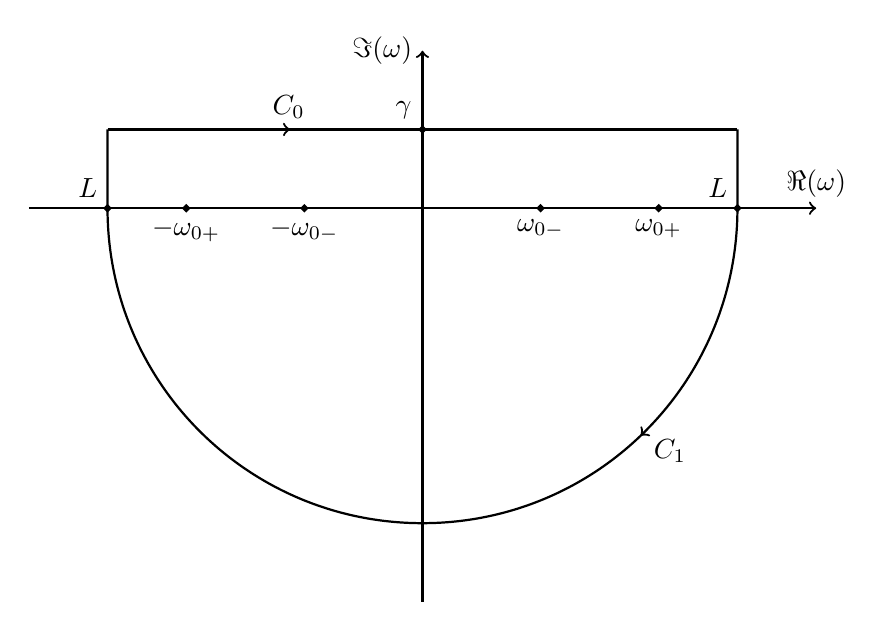
\begin{tikzpicture}[very thick,decoration={
			markings,
			mark=at position 0.29 with {\arrow{>}}}
		]
		\draw [->, thick] (-5,0) -- (5,0) node[above]{$\Re(\omega)$};
		\draw [->, thick] (0,-5) -- (0,2) node[left]{$\Im(\omega)$};
		
		\draw [postaction={decorate}, thick] (-4,1) -- (4,1);
		\draw [postaction={decorate}, thick] (4,1) to (4,0) node[above left]{$L$} to [out=-90,in=0] (0,-4) to [out=180,in=-90] (-4,0) node[above left]{$L$} to (-4,1);
		\node [above left] at (0,1) {$\gamma$};
		
		\draw[fill] (-4,0) circle [radius=0.025];
		\draw[fill] (4,0) circle [radius=0.025];
		\draw[fill] (0,1) circle [radius=0.025];
		
		\draw[fill] (3,0) circle [radius=0.025];
		\node [below] at (3,0) {$\omega_{0+}$};
		
		\draw[fill] (-3,0) circle [radius=0.025];
		\node [below] at (-3,0) {$-\omega_{0+}$};
		
		\draw[fill] (1.5,0) circle [radius=0.025];
		\node [below] at (1.5,0) {$\omega_{0-}$};
		
		\draw[fill] (-1.5,0) circle [radius=0.025];
		\node [below] at (-1.5,0) {$-\omega_{0-}$};
		
		\node [above] at (-1.7,1) {$C_0$};
		\node [below right] at (2.8,-2.8) {$C_1$};
		\end{tikzpicture} 
	}
	\caption{Bromwich contour for the complex integration of $\tilde{A}_{1,2}$.}
	\label{fig: brom cont incomp}
\end{figure}

Considering first the integral along $C_1$, we see that the integrand in question behave like $T_1(\omega)/kD(\omega) = \mathcal{O}(|\omega|^{-2})$, as $|\omega| \to \infty$. Therefore, the integral around the semi-circle vanishes, \textit{i.e.}
\begin{equation}
\lim_{L \to \infty} \int_{C_1} \frac{T_1(\omega)}{kD(\omega)} e^{-i\omega t} d\omega = 0.
\end{equation}
So we have successfully chosen a sequence of contours which limit to the same limit as that of Equation~\eqref{sol incomp}. Thankfully the integral around each of these new contours is much easier to calculate than the original, as will be exploited in the following paragraph.

Next, considering the integral along contour $C$, since it is integrated in the clockwise direction it is therefore equal to $-2\pi i$ multiplied by the sum of the residues of the singularities at $\omega = \pm \omega_{0\pm}$. The residue at $\omega = \omega_{0+}$ can be evaluated using L'Hopital's Rule (the necessary requirements ensuring the validity of this rule are verified in Appendix~\ref{app: l'hopital}), to within a free choice of initial condition, $f(x,\omega)$, as
\begin{align}
\mathrm{Res}\left[\frac{T_1(\omega)}{kD(\omega)}e^{-i\omega t}, \omega = \omega_{0+} \right] &= 
\lim_{\omega \to \omega_{0+}} \frac{(\omega - \omega_{0+})T_1(\omega)}{kD(\omega)} e^{-i\omega t} \\ 
&= \lim_{\omega \to \omega_{0+}} \frac{1}{kD'(\omega)} [T_1(\omega) + (\omega - \omega_{0+})T'_1(\omega) - it(\omega - \omega_{0+})T_1(\omega)]e^{-i\omega t} \\
&= \lim_{\omega \to \omega_{0+}} \frac{1}{kD'(\omega)} T_1\left[\omega \Psi_0 + i\frac{\partial \Psi_0}{\partial t}\right](\omega) e^{-i\omega t} \\
&= \lim_{\omega \to \omega_{0+}} \frac{1}{kD'(\omega)} \left\{ \omega T_1[\Psi_0](\omega) + iT_1\left[\frac{\partial \Psi_0}{\partial t}\right](\omega) \right\} e^{-i\omega t} \\
&= \left\{ \omega_{0+} \chi_{1+}[\Psi_0] + i\chi_{1+}\left[\frac{\partial \Psi_0}{\partial t}\right] \right\} e^{-i\omega_{0+} t},
\end{align}
where $\chi_{1+}[g] = T_1[g](\omega_{0+}) / kD'(\omega_{0+})$ is a functional mapping the function $g$ to the real numbers. In the following, we define $\chi_{1-}[g] = T_1[g](\omega_{0-}) / kD'(\omega_{0-})$, and similar for subscripts $0$ and $2$. Similarly, the residues at $\omega = -\omega_{0+}$ and $\omega = \pm\omega_{0-}$ are
\begin{align}
\mathrm{Res}\left[\frac{T_1(\omega)}{kD(\omega)}e^{-i\omega t}, \omega = -\omega_{0+} \right] &= \left\{ \omega_{0+} \chi_{1+}[\Psi_0] - i\chi_{1+}\left[\frac{\partial \Psi_0}{\partial t}\right] \right\} e^{i\omega_{0+} t}, \\
\mathrm{Res}\left[\frac{T_1(\omega)}{kD(\omega)}e^{-i\omega t}, \omega = \omega_{0-} \right] &= \left\{ \omega_{0-} \chi_{1-}[\Psi_0] + i\chi_{1-}\left[\frac{\partial \Psi_0}{\partial t}\right] \right\} e^{-i\omega_{0-} t}, \\
\mathrm{Res}\left[\frac{T_1(\omega)}{kD(\omega)}e^{-i\omega t}, \omega = -\omega_{0-} \right] &= \left\{ \omega_{0-} \chi_{1-}[\Psi_0] - i\chi_{1-}\left[\frac{\partial \Psi_0}{\partial t}\right] \right\} e^{i\omega_{0-} t}, \\
\end{align}
respectively. In the above derivation, we have used the fact that $D'$ is an odd function of $\omega$, and $D$ and $T_1[g]$ are even functions of $\omega$ for any function $g$ that does not depend on $\omega$.

Putting all of the above results together, we find that solution of the first ILT of Equation~\eqref{sol incomp}, or equivalently the boundary velocity, is
\begin{align}
\mathcal{L}^{-1}\left\{ \tilde{A}_1 \right\} &= \frac{1}{2\pi} \lim_{L \to \infty} \int_{C_0} \frac{T_1(\omega)}{kD(\omega)} e^{-i\omega t} d\omega \\
&= \frac{1}{2\pi} \lim_{L \to \infty} \int_{C} \frac{T_1(\omega)}{kD(\omega)} e^{-i\omega t} d\omega \\
&= -i \sum \mathrm{Res}\left[\frac{T_1(\omega)}{kD(\omega)}e^{-i\omega t}, \omega = \pm \omega_{0\pm} \right] \\
&= -i \left[\omega_{0+}\chi_{1+}[\Psi_0] (e^{-i\omega_{0+} t} + e^{i\omega_{0+} t}) + i\chi_{1+}\left[ \frac{\partial \Psi_0}{\partial t} \right] (e^{-i\omega_{0+} t} - e^{i\omega_{0+} t}) \right. \\
& \qquad\quad \left. + \omega_{0-}\chi_{1-}[\Psi_0] (e^{-i\omega_{0-} t} + e^{i\omega_{0-} t}) + i\chi_{1-}\left[ \frac{\partial \Psi_0}{\partial t} \right] (e^{-i\omega_{0-} t} - e^{i\omega_{0-} t})\right] \\
&= -2 \left[ i\omega_{0+}\chi_{1+}[\Psi_0] \cos(\omega_{0+} t) - \chi_{1+}\left[ \frac{\partial \Psi_0}{\partial t} \right] \sin(\omega_{0+} t) \right. \\
& \qquad\quad \left. + i\omega_{0-}\chi_{1-}[\Psi_0] \cos(\omega_{0-} t) - \chi_{1-}\left[ \frac{\partial \Psi_0}{\partial t} \right] \sin(\omega_{0-} t) \right].
\end{align}


The second ILT in Equation~\eqref{sol incomp}, $\mathcal{L}^{-1}\{ \omega / \e_1 \}$, is calculated as follows.
\begin{equation}
\mathcal{L}^{-1}\left\{ \frac{\omega}{\e_1} \right\} = \frac{1}{2\pi}\lim_{L \to \infty} \int_{i\gamma - L}^{i\gamma + L} \frac{\omega e^{-i\omega t}}{\e_1} d\omega,
= \frac{1}{2\pi\rho_1}\lim_{L \to \infty} \int_{i\gamma - L}^{i\gamma + L} \frac{\omega e^{-i\omega t}}{(kv_{A1} + \omega)(kv_{A1} - \omega)} d\omega,
\end{equation}
whose integrand has 2 simple poles at $\omega = \pm k v_{A1}$. By noting that the integrand approaches zero as $\omega \to \infty$, we can construct a Bromwich contour as shown in Figure~\ref{fig: brom cont incomp 2}. The residues of the integrand at the simple poles are
\begin{align}
\mathrm{Res}\left[\frac{\omega e^{-i\omega t}}{k^2v_{A1}^2 - \omega^2}, \omega = kv_{A1} \right] &= 
\lim_{\omega \to kv_{A1}} \frac{(\omega - kv_{A1}) \omega e^{-i\omega t}}{k^2v_{A1}^2 - \omega^2} \\ 
&= -\frac{e^{-ikv_{A1} t}}{2}, \\
\mathrm{Res}\left[\frac{\omega e^{-i\omega t}}{k^2v_{A1}^2 - \omega^2}, \omega = -kv_{A1} \right] &= 
\lim_{\omega \to -kv_{A1}} \frac{(\omega + kv_{A1}) \omega e^{-i\omega t}}{k^2v_{A1}^2 - \omega^2} \\ 
&= -\frac{e^{ikv_{A1} t}}{2}.
\end{align}
Therefore, the second ILT in Equation~\eqref{sol incomp} is
\begin{equation}
\mathcal{L}^{-1}\left\{ \frac{\omega}{\e_1} \right\} = -\frac{i}{\rho_1} \sum \mathrm{Res} \left[ \frac{\omega e^{-i\omega t}}{k^2v_{A1}^2 - \omega^2}, \omega = \pm kv_{A1} \right] = \frac{i}{\rho_1}\cos{kv_{A1}t}.
\end{equation}

Similarly, the third and final ILT in Equation~\eqref{sol incomp}, $\mathcal{L}^{-1}\{ 1 / \e_1 \}$, is calculated as follows.
\begin{equation}
\mathcal{L}^{-1}\left\{ \frac{1}{\e_1} \right\} = \frac{1}{2\pi}\lim_{L \to \infty} \int_{i\gamma - L}^{i\gamma + L} \frac{e^{-i\omega t}}{\e_1} d\omega,
= \frac{1}{2\pi\rho_1}\lim_{L \to \infty} \int_{i\gamma - L}^{i\gamma + L} \frac{e^{-i\omega t}}{(kv_{A1} + \omega)(kv_{A1} - \omega)} d\omega,
\end{equation}
whose integrand has 2 simple poles at $\omega = \pm k v_{A1}$. By noting that the integrand approaches zero as $\omega \to \infty$, we can construct a Bromwich contour as shown in Figure~\ref{fig: brom cont incomp 2}. The residues of the integrand at the simple poles are
\begin{align}
\mathrm{Res}\left[\frac{e^{-i\omega t}}{k^2v_{A1}^2 - \omega^2}, \omega = kv_{A1} \right] &= 
\lim_{\omega \to kv_{A1}} \frac{(\omega - kv_{A1}) e^{-i\omega t}}{k^2v_{A1}^2 - \omega^2} \\ 
&= -\frac{e^{-ikv_{A1} t}}{2kv_{A1}}, \\
\mathrm{Res}\left[\frac{\omega e^{-i\omega t}}{k^2v_{A1}^2 - \omega^2}, \omega = -kv_{A1} \right] &= 
\lim_{\omega \to -kv_{A1}} \frac{(\omega + kv_{A1}) e^{-i\omega t}}{k^2v_{A1}^2 - \omega^2} \\ 
&= \frac{e^{ikv_{A1} t}}{2kv_{A1}}.
\end{align}
Therefore, the final ILT in Equation~\eqref{sol incomp} is
\begin{equation}
\mathcal{L}^{-1}\left\{ \frac{1}{\e_1} \right\} = -\frac{i}{\rho_1} \sum \mathrm{Res} \left[ \frac{e^{-i\omega t}}{k^2v_{A1}^2 - \omega^2}, \omega = \pm kv_{A1} \right] = \frac{\sin{kv_{A1}t}}{\rho_1kv_{A1}}.
\end{equation}

\begin{figure}
	\centering
	\scalebox{0.9}{
		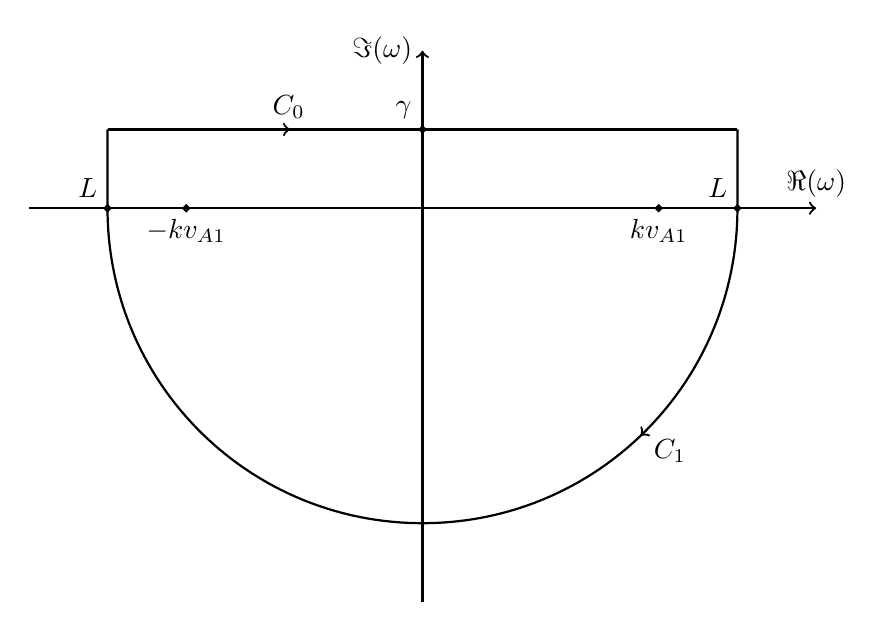
\begin{tikzpicture}[very thick,decoration={
			markings,
			mark=at position 0.29 with {\arrow{>}}}
		]
		\draw [->, thick] (-5,0) -- (5,0) node[above]{$\Re(\omega)$};
		\draw [->, thick] (0,-5) -- (0,2) node[left]{$\Im(\omega)$};
		
		\draw [postaction={decorate}, thick] (-4,1) -- (4,1);
		\draw [postaction={decorate}, thick] (4,1) to (4,0) node[above left]{$L$} to [out=-90,in=0] (0,-4) to [out=180,in=-90] (-4,0) node[above left]{$L$} to (-4,1);
		\node [above left] at (0,1) {$\gamma$};
		
		\draw[fill] (-4,0) circle [radius=0.025];
		\draw[fill] (4,0) circle [radius=0.025];
		\draw[fill] (0,1) circle [radius=0.025];
		
		\draw[fill] (3,0) circle [radius=0.025];
		\node [below] at (3,0) {$kv_{A1}$};
		
		\draw[fill] (-3,0) circle [radius=0.025];
		\node [below] at (-3,0) {$-kv_{A1}$};
		
		\node [above] at (-1.7,1) {$C_0$};
		\node [below right] at (2.8,-2.8) {$C_1$};
		\end{tikzpicture} 
	}
	\caption{Bromwich contour for the complex integration of the integrand of $J_1$.}
	\label{fig: brom cont incomp 2}
\end{figure}
Combining the above expressions we find that the transverse velocity solution for $x<-x_0$ is
\begin{align}
v_x = &-2 e^{k(x+x_0)} \left\{ i\omega_{0+}\chi_{1+}[\Psi_0] \cos(\omega_{0+} t) - \chi_{1+}\left[ \frac{\partial \Psi_0}{\partial t} \right] \sin(\omega_{0+} t) + i\omega_{0-}\chi_{1-}[\Psi_0] \cos(\omega_{0-} t) - \chi_{1-}\left[ \frac{\partial \Psi_0}{\partial t} \right] \sin(\omega_{0-} t) \right\} \\
&+ \frac{i}{\rho_1} \int_{-\infty}^{-x_0} G_1(x;s) \left[ \Psi(s, 0) \cos{kv_{A1}t} + \frac{\partial \Psi}{\partial t}(s, 0) \frac{\sin{kv_{A1}t}}{kv_{A_1}} \right]ds.
\end{align}
Similarly, the transverse velocity for the region $x>x_0$ is
\begin{align}
v_x &= \mathcal{L}^{-1} \left\{ \tilde{A}_2e^{k(x_0-x)} + \frac{1}{\e_2} \int_{x_0}^{\infty} G_2(x;s)f(s, \omega)ds \right\}, \\
&= e^{k(x_0-x)} \mathcal{L}^{-1}\left\{ \tilde{A}_2 \right\} + \int_{x_0}^{\infty} G_2(x;s)\mathcal{L}^{-1}\left\{ \frac{f(s, \omega)}{\e_2} \right\} ds, \\
&= -2 e^{k(x_0 - x)} \left\{ i\omega_{0+}\chi_{2+}[\Psi_0] \cos(\omega_{0+} t) - \chi_{2+}\left[ \frac{\partial \Psi_0}{\partial t} \right] \sin(\omega_{0+} t) + i\omega_{0-}\chi_{2-}[\Psi_0] \cos(\omega_{0-} t) - \chi_{2-}\left[ \frac{\partial \Psi_0}{\partial t} \right] \sin(\omega_{0-} t) \right\} \\
& \quad + \frac{i}{\rho_2} \int_{x_0}^{\infty} G_2(x;s) \left[ \Psi(s, 0) \cos{kv_{A2}t} + \frac{\partial \Psi}{\partial t}(s, 0) \frac{\sin{kv_{A2}t}}{kv_{A_2}} \right]ds.
\end{align}
Finally, for the region $|x|<x_0$, it is
\begin{align}
v_x =& \mathcal{L}^{-1} \left\{ \frac{1}{\sinh{2kx_0}} \left[ \tilde{A}_1\sinh(k(x_0 - x)) + \tilde{A}_2\sinh(k(x_0 + x)) \right] + \frac{1}{\epsilon_0}\int_{-x_0}^{x_0} G_0(x;s) f(s, \omega) ds \right\}, \\
=& \frac{1}{\sinh{2kx_0}} \left[\mathcal{L}^{-1}\{\tilde{A}_1\} \sinh(k(x_0 - x)) + \mathcal{L}^{-1}\{\tilde{A}_2\} \sinh(k(x_0 + x)) \right] + \int_{-x_0}^{x_0} G_0(x;s) \mathcal{L}^{-1}\left\{\frac{f(s, \omega)}{\e_0} \right\} ds, \\
=& -\frac{2}{\sinh{2kx_0}} \left[ \left\{ i\omega_{0+}\chi_{1+}[\Psi_0] \cos(\omega_{0+} t) - \chi_{1+}\left[ \frac{\partial \Psi_0}{\partial t} \right] \sin(\omega_{0+} t) + i\omega_{0-}\chi_{1-}[\Psi_0] \cos(\omega_{0-} t) - \chi_{1-}\left[ \frac{\partial \Psi_0}{\partial t} \right] \sin(\omega_{0-} t) \right\} \sinh(k(x_0 - x)) \right. \\ 
&+ \left. \left\{ i\omega_{0+}\chi_{2+}[\Psi_0] \cos(\omega_{0+} t) - \chi_{2+}\left[ \frac{\partial \Psi_0}{\partial t} \right] \sin(\omega_{0+} t) + i\omega_{0-}\chi_{2-}[\Psi_0] \cos(\omega_{0-} t) - \chi_{2-}\left[ \frac{\partial \Psi_0}{\partial t} \right] \sin(\omega_{0-} t) \right\} \sinh(k(x_0 + x)) \right] \notag \\
& + \frac{i}{\rho_0} \int_{-x_0}^{x_0} G_0(x;s) \left[ \Psi(s, 0) \cos{kv_{A0}t} + \frac{\partial \Psi}{\partial t}(s, 0) \frac{\sin{kv_{A0}t}}{kv_{A0}} \right]ds.
\end{align}


\subsection{Specific initial conditions}

\subsubsection{Uniform initial vorticity}

Let $\Omega(x, 0) = \Omega_0$ be constant. Therefore, $\Psi_0 = k\rho_0\Omega_0$ and $\partial \Psi_0 / \partial t = 0$. To evaluate the solution, we evaluate each Green's function integral separately:
	\begin{align}
	\int_{-\infty}^{-x_0} G_1(x;s) \Psi_0 ds &= \Omega_0 \rho_1 \left[ \sinh(k(x+x_0)) \int_{-\infty}^{x} e^{k(s + x_0)} ds + e^{k(x+x_0)} \int_{x}^{-x_0} \sinh(k(s+x_0)) ds \right], \\
	&= \frac{\Omega_0 \rho_1}{k} \left[ e^{k(x+x_0)} - 1 \right].
	\end{align}
	
	\begin{align}
	\int_{-x_0}^{x_0} G_0(x;s) \Psi_0 ds &= \Omega_0 \rho_0 \left[ \sinh(k(x-x_0)) \int_{-x_0}^{x} \sinh(k(s+x_0)) ds + \sinh(k(x+x_0)) \int_{x}^{x_0} \sinh(k(s-x_0)) ds \right], \\
	&= 0.
	\end{align}
	
	\begin{align}
	\int_{x_0}^{\infty} G_2(x;s) \Psi_0 ds &= - \Omega_0 \rho_2 \left[ e^{-k(x-x_0)} \int_{x_0}^{x} \sinh(k(s-x_0)) ds + \sinh(k(x-x_0)) \int_{x}^{\infty} e^{-k(s-x_0)} ds \right], \\
	&= \frac{\Omega_0 \rho_2}{k} \left[ e^{-k(x-x_0)} - 1 \right].
	\end{align}

\begin{align}
I_0^\pm &= \frac{\Omega_0\omega\rho_0k}{\sinh{2kx_0}} \int_{-x_0}^{x_0} \sinh(k(s \pm x_0)) ds, \\
&= \pm \frac{\Omega_0 \omega \rho_0}{\sinh{2kx_0}} (\cosh{2kx_0 - 1}).
\end{align}

\begin{align}
I_1 &= \Omega_0\omega\rho_1k \int_{-\infty}^{-x_0} e^{k(s + x_0)} ds, \\
&= \Omega_0 \omega \rho_1.
\end{align}

\begin{align}
I_2 &= \Omega_0\omega\rho_2k \int_{x_0}^{\infty} e^{k(x_0 - s)} ds, \\
&= \Omega_0 \omega \rho_2.
\end{align}
Using the above, the transverse velocity through time for an initially constant vorticity is
\begin{equation}
v_x = -\frac{i}{k}\begin{cases}
2 e^{k(x+x_0)} A^*_1 + \Omega_0 \{1 - e^{k(x+x_0)}\} \cos{kv_{A1}t} \quad &\text{ for } x<-x_0, \\
\frac{2}{\sinh{2kx_0}} \left[ A^*_1 \sinh(k(x_0 - x)) + A^*_2 \sinh(k(x_0 + x)) \right] \quad &\text{ for } x<|x_0|, \\
2 e^{k(x_0-x)} A^*_2 + \Omega_0 \{1 - e^{k(x_0-x)}\} \cos{kv_{A2}t} \quad &\text{ for } x>x_0, \\
\end{cases}
\end{equation}
where
\begin{align}
A^*_1 &= \omega_{0+} \frac{T_1[\psi_0](\omega_{0+})}{D'(\omega_{0+})} \cos(\omega_{0+} t) + \omega_{0-}\frac{T_1[\psi_0](\omega_{0-})}{D'(\omega_{0-})} \cos(\omega_{0-} t), \\
A^*_2 &= \omega_{0+} \frac{T_2[\psi_0](\omega_{0+})}{D'(\omega_{0+})} \cos(\omega_{0+} t) + \omega_{0-}\frac{T_2[\psi_0](\omega_{0-})}{D'(\omega_{0-})} \cos(\omega_{0-} t), \\
\end{align}
and
\begin{equation}
T_{1,2}[\Psi_0](\omega) = -\Omega_0\{ (\rho_0 \tanh{kx_0} + \rho_{1,2}) (\e_0 \cosh{2kx_0} + \e_{2,1}\sinh{2kx_0}) + \e_0(\rho_0 \tanh{kx_0} + \rho_{2,1}) \}.
\end{equation}


\subsubsection{Corroboration with interface}
When $\rho_1 = \rho_2 = \rho_0$,
\begin{equation}
T_{1,2}[\Psi_0](\omega) = -2\Omega_0\rho_0 e^{kx_0} (\e_0 \cosh{kx_0} + \e_{2,1}\sinh{kx_0}).
\end{equation}

When $\rho_1 = \rho_2 = \rho_0$ and $x_0 = 0$, we expect that the solution will reduce to (the corrected version of) Equation~(25) in \cite{rae_etal81}. Let's check that this is the case.

When the above conditions hold, the dispersion function reduces to $D(\omega) = \e_0(\e_1 + \e_2)$ and its zeroes reduce to $\omega_{0+} = kv_{A0}$ and $\omega_{0-} = kv_{AS} = k \sqrt{(v_{A1}^2 + v_{A2}^2) / 2}$. Therefore, the functionals reduce to
\begin{equation}
T_{1,2}[\Psi_0](\omega) = -2\Omega_0\rho_0 \e_0,
\quad 
\chi_{1,2}[\Psi_0](\omega_{0+}) = 0,
\quad
\chi_{1,2}[\Psi_0](\omega_{0-}) = \frac{\Omega_0}{2k^2v_{AS}}.
\end{equation}
Therefore, the transverse velocity solution reduces to
\begin{equation}
v_x = -\frac{i\Omega_0}{k} 
\begin{cases}
(1 - e^{kx})\cos{kv_{A1}t} + e^{kx}\cos{kv_{AS}t} \quad &\text{ for } x < 0, \\
(1 - e^{-kx})\cos{kv_{A2}t} + e^{-kx}\cos{kv_{AS}t} \quad &\text{ for } x > 0,
\end{cases}
\end{equation}
which corroborates with (the corrected version of) the result from \cite{rae_etal81}.

%%%%%%%%%%%%%%%%%%%%%%%%%%%%%%%%%%%%%%%%%%%%%%%%%%%%%%%%%%

\acknowledgments
M. Allcock acknowledges the support from the University Prize Scholarship at the University of Sheffield. R. Erd\'{e}lyi acknowledges the support from the UK Science and Technology Facilities Council (STFC grant number: ST/M000826/1) and the Royal Society. 

% inlude mayavi visualisations and link to the website?
%\software{Mayavi}

\appendix

\section{Non-standard Laplace transform}\label{app: laplace trans}
Consider a function $f(t)$, whose standard Laplace transform, $F_1(\omega)$, and non-standard Laplace transform, $F_2(\omega)$, are
\begin{equation}
F_1(\omega) = \int_0^\infty f(t) e^{-\omega t} dt,
\quad \text{and} \quad
F_2(\omega) = \int_0^\infty f(t) e^{i\omega t} dt.
\end{equation}
Trivially, $F_1(-i\omega) = F_2(\omega)$. Using the standard inverse Laplace transform, and letting $\gamma$ be real and greater than the real part of all the singularities of $F_1(\omega)$, the original function $f(t)$ can be written
\begin{align}
f(t) & = \frac{1}{2\pi i} \lim_{T\to\infty} \int_{\gamma - iT}^{\gamma + iT} F_1(\omega)e^{\omega t} d\omega, \\
& = \frac{1}{2\pi i} \lim_{T\to\infty} \int_{i\gamma - T}^{i\gamma + T} F_1(-i\omega)e^{-i\omega t} (-id\omega), \\
& = \frac{1}{2\pi} \lim_{T\to\infty} \int_{i\gamma - T}^{i\gamma + T} F_2(\omega)e^{-i\omega t} d\omega.
\end{align}
Therefore, the inverse transform of the non-standard Laplace transform is
\begin{equation}
f(t) = \frac{1}{2\pi} \lim_{T\to\infty} \int_{i\gamma - T}^{i\gamma + T} F_2(\omega)e^{-i\omega t} d\omega.
\end{equation}


\section{Corroboration of incompressible solutions with previous results}

\subsection{Interface}\label{app: interface}
When we let the width of an asymmetric slab vanish, we recover the traditional interface geometry. Letting $x_0 \to 0$, the parameters $a$, $b$, and $c$, from Equations~\eqref{solution a}, \eqref{solution b}, and~\eqref{solution c}, reduce to
\begin{align}
a &= \rho_0(\rho_1 + \rho_2), \\
b &= -\rho_0v_{A0}^2(\rho_1 +\rho_2) - \rho_0(\rho_1v_{A1}^2 + \rho_2v_{A2}^2), \\
c &= \rho_0v_{A0}^2(\rho_1v_{A1}^2 + \rho_2v_{A2}^2).
\end{align}
Therefore, when the slab width vanishes, the eigenmodes given by Equation~\eqref{solution omega0} reduce to
\begin{equation}
\left(\frac{\omega_0}{k}\right)^2 = \frac{-b \pm \sqrt{b^2 - 4ac}}{2a} =
\begin{cases}
v_{A0}^2, \\
\frac{\rho_1v_{A1}^2 + \rho_2v_{A2}^2}{\rho_1 + \rho_2}.
\end{cases}
\end{equation}
The first solution above is degenerate because, while the parameter $v_{A0}$ makes sense in the limit as the slab width vanishes, it is meaningless in an interface system constructed without an inner region. The second solution corroborates with the surface eigenfrequencies of an interface, as expected \citep{rob81a}.



\subsection{Symmetric slab}\label{app: symmetric}

By letting the parameters on each external plasma region be equal (\textit{i.e.} $\rho_1 = \rho_2 = \rho_e$, and similar for the magnetic field and Aflv\'{e}n speed) the asymmetric slab is reduced to a symmetric slab. In this limit, the parameters $a$, $b$, and $c$, from Equations~\eqref{solution a}, \eqref{solution b}, and~\eqref{solution c}, can be reduced to
\begin{align}
a &= \frac{2}{\tau_0 + c_0} \left[ \rho_0^2 + \rho_e^2 + \rho_0\rho_e(\tau_0 + c_0) \right], \\
b &= \frac{-2}{\tau_0 + c_0} \left[ 2(\rho_0^2v_{A0}^2 + \rho_e^2v_{Ae}^2) + \rho_0\rho_e(v_{A0}^2 + v_{Ae}^2)(\tau_0 + c_0) \right], \\
c &= \frac{2}{\tau_0 + c_0} \left[ \rho_0^2v_{A0}^4 + \rho_e^2v_{Ae}^4 + \rho_0\rho_ev_{A0}^2v_{Ae}^2(\tau_0 + c_0) \right],
\end{align}
where $\tau_0 = \tanh{kx_0}$ and $c_0 = \coth{kx_0}$. The discriminant in the solution, Equation~\eqref{solution omega0}, reduces to
\begin{equation}
b^2 - 4ac = 4\rho_0^2\rho_e^2(v_{A0}^2 - v_{Ae}^2)^2 \left(\frac{\tau_0 - c_0}{\tau_0 + c_0}\right)^2. 
\end{equation}
Therefore, the eigenfrequencies reduce to
\begin{equation}
\left(\frac{\omega_0}{k}\right)^2 = \frac{-b \pm \sqrt{b^2 - 4ac}}{2a} =
\begin{cases}
\frac{\rho_0v_{A0}^2 + \rho_ev_{Ae}^2c_0}{\rho_0 + \rho_ec_0}, \\
\frac{\rho_0v_{A0}^2 + \rho_ev_{Ae}^2\tau_0}{\rho_0 + \rho_e\tau_0},
\end{cases}
\end{equation}
which corroborates with Equation~(12) in \cite{rob81b}.


\section{Validation of L'Hopital's rule} \label{app: l'hopital}
L'Hopital's Rule is a powerful tool for evaluating limits of quotients of functions, provided that these functions satisfy certain necessary criteria. L'Hopital's Rule (for function of complex variables) states that, for functions $f$ and $g$ which are analytic at a point $z_0$, if $f(x_0) = g(z_0) = 0$, $g'(z_0) \neq 0$ then
\begin{equation}
\lim_{z \to z_0}\frac{f(z)}{g(z)} = \frac{f'(z)}{g'(z)}.
\end{equation}
There are stronger formulations of the complex L'Hopital's rule which are superfluous for our present needs \textcolor{red}{CITATION?}.

Applied to the present problem, the requirements for L'Hopital's rule to hold are:
\begin{enumerate}
	\item The functions $(\omega - \omega_{0+}) T_1(\omega) e^{-i\omega t}$ and $kD(\omega)$ are analytic at $\omega_{0+}$,
	\item $[(\omega - \omega_{0+}) T_1(\omega) e^{-i\omega t}]|_{\omega = \omega_{0+}} = kD(\omega_{0+}) = 0$,
	\item $kD'(\omega_{0+}) \neq 0$.
\end{enumerate}

Below, we validate that each of these conditions holds:
\begin{enumerate}
	\item Functions $T_1(\omega)$ and $D(\omega)$ are polynomials and hence are analytic. Since products of analytic functions are also analytic, $(\omega - \omega_{0+}) T_1(\omega) e^{-i\omega t}$ and $kD(\omega)$ are analytic. In particular, they are analytic at $\omega_{0+}$.
	
	\item The point $\omega_{0+}$ is a zero of $D(\omega)$ (by definition of $\omega_{0+}$) and $T_1(\omega)$ is regular at $\omega_{0+}$, therefore $[(\omega - \omega_{0+}) T_1(\omega) e^{-i\omega t}]|_{\omega = \omega_{0+}} = kD(\omega_{0+}) = 0$.
	
	\item The function $D'(\omega)$ can be rewritten as
	\begin{align}
	D'(\omega) &= 2k^2\omega\left[ 2\{c_0\rho_0(\rho_1 + \rho_2) + s_0(\rho_0^2 + \rho_1\rho_2)\}\frac{\omega^2}{k^2} \right. \notag \\
	& \qquad \qquad - \left. \{c_0\rho_0[\rho_1v_{A1}^2 + \rho_2v_{A2}^2 + (\rho_1 + \rho_2)v_{A0}^2] + s_0[2\rho_0^2v_{A0}^2 + \rho_1\rho_2(v_{A1}^2 + v_{A2}^2)]\}\right] \\
	& = 2k^2\omega\left[ 2a \frac{\omega^2}{k^2} + b \right],
	\end{align}
	where $a$ and $b$ are given by Equations~\eqref{solution a} and~\eqref{solution b}. The above equation has zeros at $\omega = 0$ and $\omega = \pm \omega_0$, where
	\begin{equation}
	\frac{\omega_0^2}{k^2} = -\frac{b}{2a}.
	\end{equation}
	Therefore, the zeros of the function $D$ are always at least a factor of $i$ away from the zeros of $D'$ (and are a factor of exactly $i$ away if and only if $d = b^2 - 4ac = 0$). The result follows.
\end{enumerate}



%%%%%%%%%%%%%%%%%%%%%%%%%%%%%%%%%%%%%%%%%%%%%%%%%%%%%

\bibliography{Bibliography}

\end{document}
